\documentclass[12pt]{report}

\usepackage[T1]{fontenc}
\usepackage[utf8]{inputenc}
\usepackage{graphicx}
\usepackage{amsmath,amssymb,amsfonts}
\usepackage{txfonts}
\usepackage{pdfpages}
\usepackage{caption}
\usepackage{float}
\usepackage{listings}

\renewcommand{\chaptername}{Rozdział}
\renewcommand{\contentsname}{Spis treści}
\renewcommand{\figurename}{Rys.}
\renewcommand{\tablename}{Tab.}
\renewcommand{\listfigurename}{Spis rysunków}
\renewcommand{\listtablename}{Spis tabel}
\renewcommand{\bibname}{Bibliografia}
\renewcommand\lstlistingname{Listing}
\renewcommand\lstlistlistingname{Spis listingów}

\pagestyle{headings}

\setlength{\textwidth}{14cm}
\setlength{\textheight}{20cm}

\newtheorem{definition}{Definicja}
\newtheorem{example}{Przykład}[chapter]
\newtheorem{corollary}{Wniosek}[chapter]

\begin{document}

\lstdefinestyle{customcmd}{
captionpos=b, 
belowcaptionskip=1\baselineskip,
breaklines=true,
frame=LRTB,
xleftmargin=\parindent,
showstringspaces=false,
basicstyle=\footnotesize\ttfamily
}

\lstdefinestyle{customsql}{
captionpos=b, 
belowcaptionskip=1\baselineskip,
breaklines=true,
frame=LRTB,
xleftmargin=\parindent,
language=SQL,
showstringspaces=false,
basicstyle=\footnotesize\ttfamily,
keywordstyle=\bfseries\color{purple},
identifierstyle=\color{violet}
}

\lstdefinestyle{customc}{
captionpos=b, 
belowcaptionskip=1\baselineskip,
breaklines=true,
frame=LRTB,
xleftmargin=\parindent,
language=C++,
showstringspaces=false,
basicstyle=\footnotesize\ttfamily,
keywordstyle=\bfseries\color{green!40!black},
commentstyle=\itshape\color{purple!40!black},
identifierstyle=\color{blue},
stringstyle=\color{orange},
}

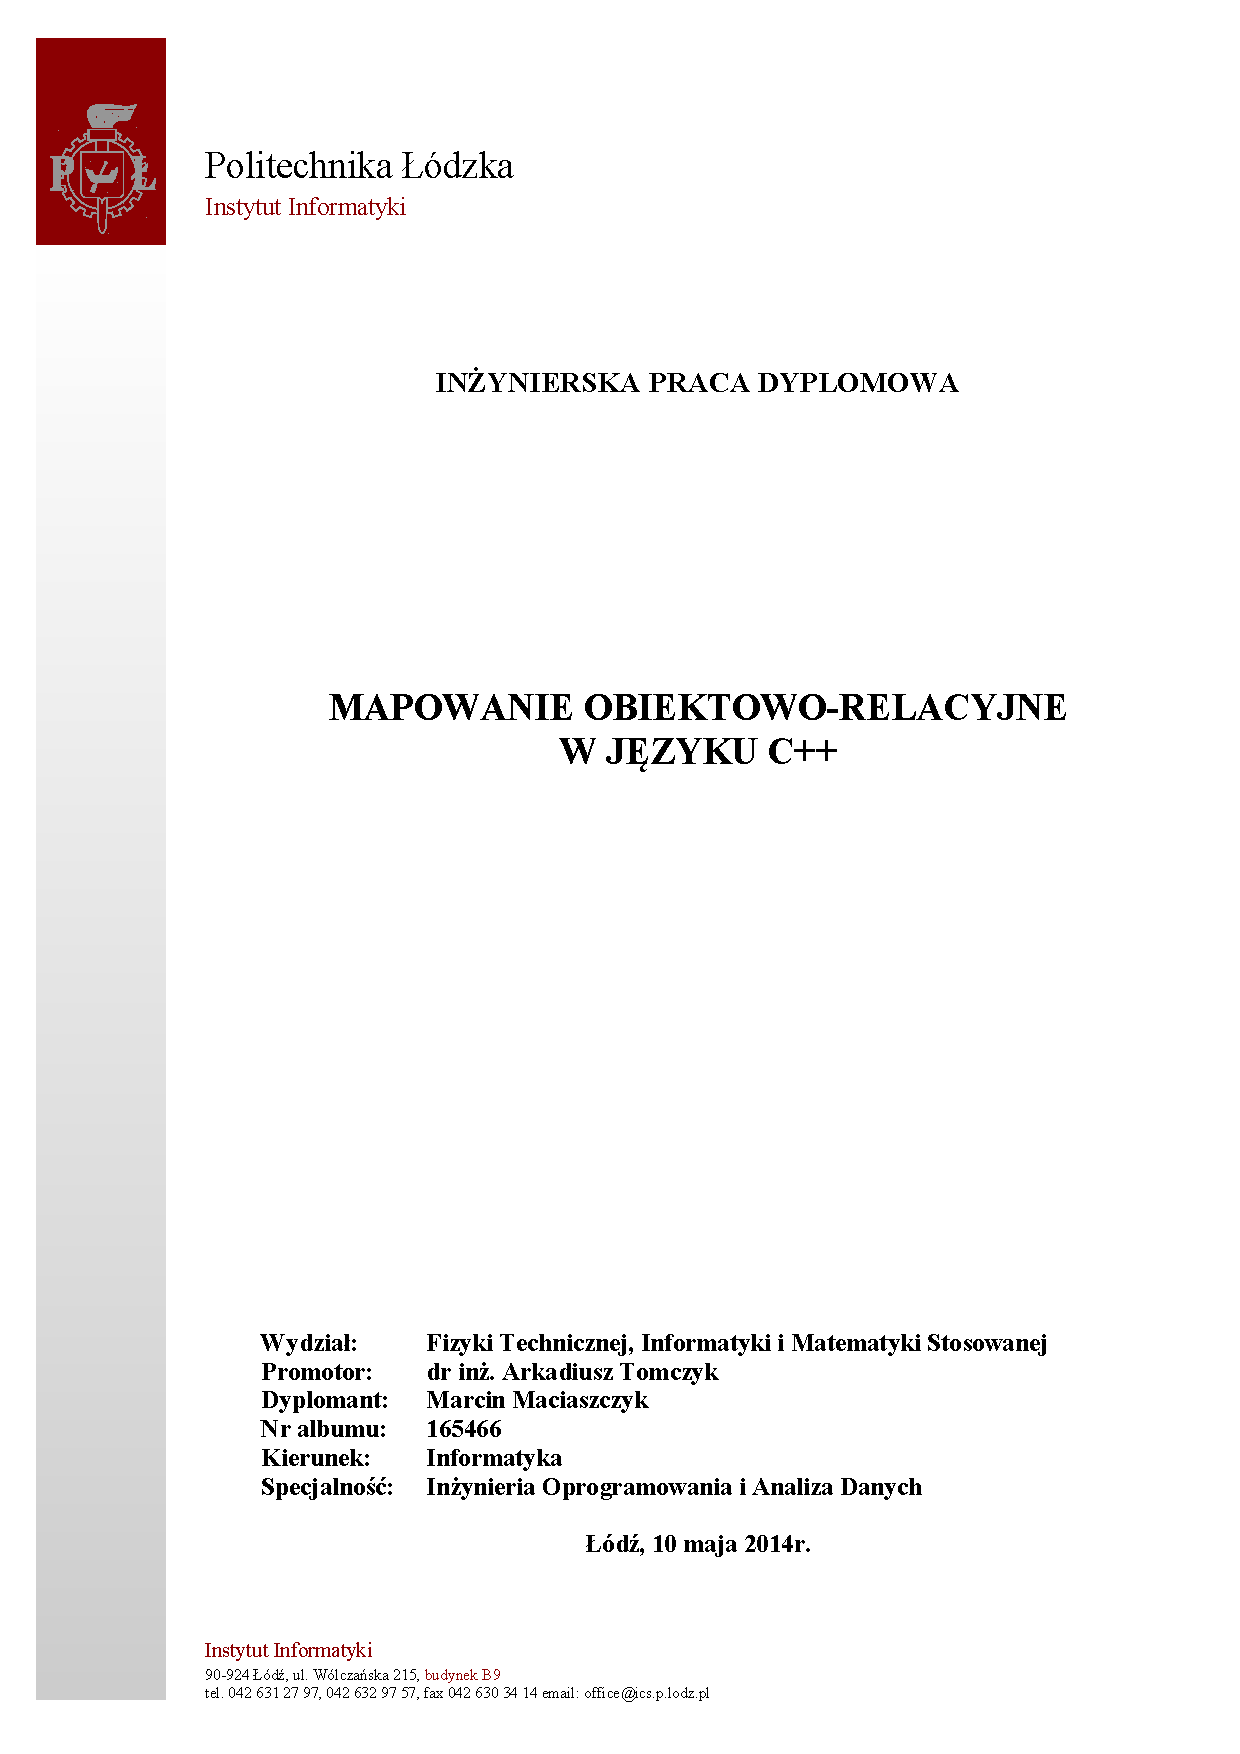
\includepdf[pages={1}]{resources/title_page.pdf}

\tableofcontents

\chapter{Wstęp} \label{wstep}

\section{Uzasadnienie wyboru tematu}

Wraz z rozwojem informatyki proces tworzenia oprogramowania wymaga od informatyków co raz większej wiedzy w poszczególnych dziedzinach takich jak na przykład bazy 
danych czy sieci komputerowe. Ciężko jest być specjalistą w każdej z nich, dlatego też podczas tworzenia oprogramowania programiści co raz częściej sięgają po różnego 
rodzaju narzędzia programistyczne, które mają za zadanie uła\-twić im pracę, wykonując jej część za nich.

Przykładem wspomnianych narzędzi programistycznych są aplikacje szkieletowe wykorzystywane jako fundamenty dla tworzonych aplikacji czy też biblioteki programistyczne
udostępniające zestawy funkcji związanych z wybranym zagadnieniem. Nie zawsze mamy możliwość skorzystania z nich, jednak jeśli taka istnieje warto to rozważyć,
ponieważ podejmując decyzję o ich wykorzystaniu powstaje możliwość zaoszczędzenia sporej ilości czasu, który można poświęcić na rozwią\-zanie postawionego przed nami
głównego problemu biznesowego, a także uniknąć wielu błędów związanych z nieznajomością danej dziedziny.

Autor tej pracy wraz z kolegą z roku studiów -- Sebastianem Florkiem, w ramach pisania pracy dyplomowej zdecydował się na współpracę przy tworzeniu wspólnej aplikacji
szkieletowej, której zadaniem będzie realizowanie mapowania obiektowo-relacyjnego w języku C++. Wybór języka programowania autorzy tłumaczą dobrą jego 
znajomością nabytą w trakcie trwania studów. Główny przedmiot pracy, czyli mapowanie obiektowo-relacyjne to obecnie zagadnienie co raz bardziej powszechne, 
szczególnie w językach programowania takich jak PHP czy Java. Programiści C++ nie mają już tak dużego wyboru wśród dostępnych narzędzi służących do mapowania 
obiektowo-relacyjnego, co także miało znaczenie podczas wyboru zagadnienia które niniejsza praca ma podejmować.

\begin{figure}[H]
\centering
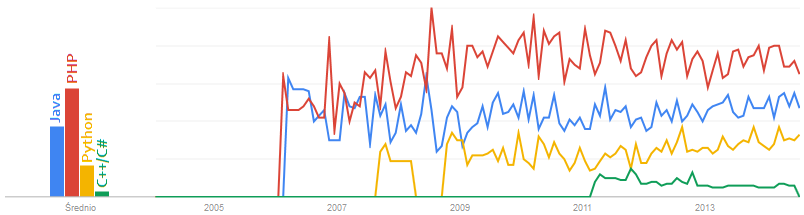
\includegraphics[width=\textwidth]{resources/trends.png}
\caption[Wykres przedstawiający popularność mapowania obiektowo-relacyjnego na przestrzeni czasu w wybranych językach programowania] {Wykres przedstawiający 
popularność mapowania obiektowo-relacyjnego na przestrzeni czasu w wybranych językach programowania \cite{trends}}
\end{figure}

Podział pracy współautorów tworzonej aplikacji szkieletowej, dalej pojawiającej się także pod nazwą Qubic, był kluczową kwestią do ustalenia. Ostatecznie przyjęty został
on w sposób następujący -- tematem pracy Sebastiana jest ,,Generowanie opisu mapowania obiektowo-relacyjnego w języku C++'' i to właśnie stworzenie generatora opisu
mapowania jest głównym celem badawczym jego pracy. Zgodnie z tytułem tej pracy, jej autor będzie zajmował zrealizowaniem samego mapowania obiektowo-relacyjnego.
Zadaniem generatora będzie wygenerowanie opisu mapowania w postaci plików nagłówkowych, klas oraz pliku projektu. Drugi moduł natomiast będzie implementował 
mapowanie obiektowo-relacyjne w wygenerowanych plikach oraz udostępniał interfejs dostępny dla użytkownika.

\begin{figure}[h]
\centering
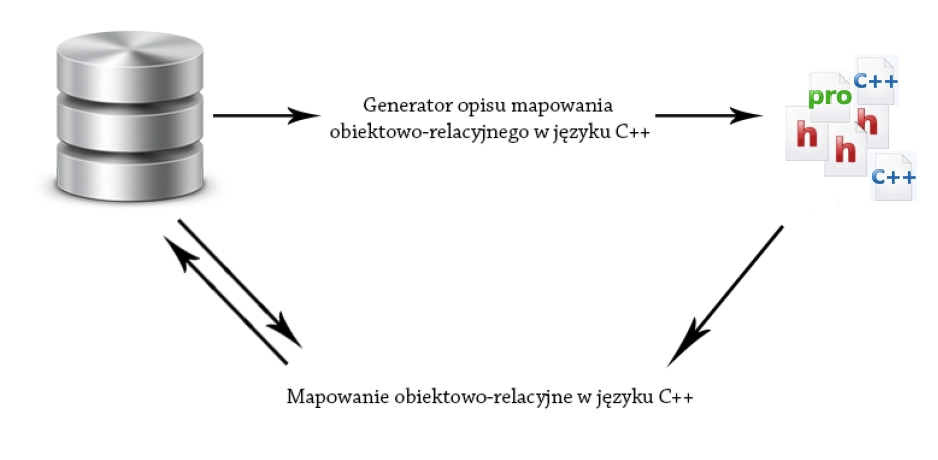
\includegraphics[width=\textwidth]{resources/coop.png}
\caption[Schemat współpracy modułów tworzonej aplikacji szkieletowej]{Schemat współpracy modułów tworzonej aplikacji szkieletowej, dalej występującej też pod nazwą Qubic}
\end{figure}

\section{Problematyka i zakres pracy}

Programowanie obiektowe jest obecnie jednym z najpopularniejszych pa\-ra\-dy\-gma\-tów programowania, a pojęcia takie jak klasa czy obiekt znane są wszystkim programistom.
Podobnie jest z relacyjnym modelem organizacji baz danych i terminami takimi jak relacja czy krotka. Chcąc wykorzystać oba te podejścia w jednej aplikacji musimy zadbać o 
obustronną konwersję pomiędzy danymi z tabel relacyjnej bazy danych a obiektami aplikacjii. Tym właśnie zajmuje się mapowanie obiektowo-relacyjne, które wraz z tworzeniem 
aplikacji szkieletowych w języku C++ jest główną problematyką niniejszej pracy.

Tutaj powstaje pytanie czy na prawdę warto korzystać z bibliotek i aplikacji szkieletowych służących do mapowania obiektowo relacyjnego? Od\-po\-wiedź nie jest
jednoznaczna w wszystkich przypadkach, ale warto wymienić jego podstawowe wady i zalety, których dokładniejsza analiza znajduje się w dalszej części pracy. Zacznijmy od zalet 
wykorzystania narzędzi ORM\footnote{~mapowanie obiektowo-relacyjne (ang. Object-Relational Mapping)}:

\begin{itemize}
\item Oszczędność -- znacznie zredukowana zostaje ilość pracy wymagana na oprogramowanie dostępu do bazy danych.
\item Uniezależnienie się od rodzaju systemu zarządzania bazą danych -- możliwość korzystania z wielu rozdzajów baz danych, a także możliwość jego zmiany w dowolnym
momencie bez ponoszenia większych strat czasowych.
\item Nieobowiązkowa znajomość języka SQL\footnote{~strukturalny język zapytań (ang. Structured Query Language)} -- w celu tworzenia zapytań do bazy wykorzystywany
jest udostępniany interfejs.
\item Liczne funkcjonalności -- aby skorzystać z transakcji, połączenia z bazą danych a także wieu innych funkcjonalności baz danych wystarczy zazwyczaj wywołać
pojedyńczą metodę.
\item Model danych przechowywany w jednym miejscu -- dzięki czemu łatwiej jest zarządzać kodem.
\end{itemize}

W parze z przedstawionymi zaletami pojawiają się także pewne wady:

\begin{itemize}
\item Konfiguracja jest najczęściej skomplikowana i wymaga sporo czasu.
\item Aby efektownie korzystać z narzędzi do mapowania obiektowo-relacyjnego wymagana jest ich dobra znajomość.
\item Proste zapytania są obsługiwane bardzo sprawnie, jednak gdy przetwarzamy duże ilości złożonych zapytań wydajność nie dorówna nigdy zapytaniom na\-pi\-sa\-nym
przez specjalistę znającego język SQL.
\item Abstrakcja wprowadzona przez narzędzia ORM może okazać się uciążliwa, ponieważ nie zawsze zdajemy sobie sprawę z tego co dzieje się za kulisami w trakcie
wykonywania poszczególnch operacji.
\end{itemize}

Głównym celem autorów Qubica jest sprawienie aby stał się on dobrą alternaty\-wą dla nielicznych, ale istniejących już narzędzi realizujących mapowanie obiekt\-owo-relacyjne 
w języku C++. Wszystkie znane rozwiązania są dostępne za darmo, jednak albo nie udostępniają one generatora opisu będącego w stanie  wygenerować cały projekt aplikacji
albo ich interfejsy nie należą do intuicyjnych. Wprowadzenie generatora oraz intuicyjnego interfejsu użytkownika powinno uczynić Qubica istotną alternatywą dla istniejących już
narzędzi za\-kła\-da\-jąc, że pozostała funkcjonalność mapowania obiektowo-relacyjnego zostanie zre\-al\-iz\-owana poprawnie.

\section{Cele pracy}

Do najważniejszych celów niniejszej pracy dyplomowej należą:

\begin{itemize}
\item Analiza istniejących bibliotek programistycznych realizujących ma\-po\-wa\-nie obiektowo-relacyjne w języku C++ -- przeanalizowanie istniejących już na\-rzędzi
umożliwi dokładniejsze zapoznanie się z tematyką mapowania obiekt\-owo-relacyjnego a także ze sposobem działania istniejących już rozwiązań, co umożliwi wykorzystanie 
najciekawszych pomysłów w Qubicu a także wskaże elementy, które mogą ulec w nim poprawie.
\item Stworzenie własnej aplikacji szkieletowej realizującej mapowanie obiektowo-relacyjne w języku C++ -- ułatwi dokładniejsze poznanie mechanizmów dzia\-łających
podczas mapowania obiektowo-relacyjnego oraz sposobów ro\-zwią\-zania pojawiających się problemów.
\item Porównanie Qubica z wcześniej analizowanymi narzędziami -- porównanie to pozwoli stwierdzić czy przyjęte założenia i zastosowane rozwiązania okazały się słuszne
oraz czy Qubic wnosi coś nowego do grona istniejących rozwiązań.
\end{itemize}

\newpage

Do celów części praktycznej należą:

\begin{itemize}
\item Stworzenie intuicyjnego interfejsu użytkownika -- im mniej linii kodu musi zostać napisane w celu wykonania podstawowych operacji bazodanowych tym interfejs jest 
uważany za bardziej intuicyjny.
\item Stworzenie generatora opisu mapowania obiektowo-relacyjnego -- jest to celem pracy Sebastiana. Wspólnym celem obu autorów jest integracja utworzonych  modułów.
\item Poprawne zrealizowanie założeń mapowania obiektowo-relacyjnego, a także jak najlepsza optymalizacja zapytań -- mapowanie musi odbywać się możliwie szybko, jednak
najważniejsze jest zrealizowanie wszystkich jego założeń.
\item Uczynienie konfiguracji Qubica jak najprostszą -- najlepszym rozwiązaniem wydaje się być przeniesienie całej konfiguracji do pliku konfiguracyjnego, tak aby nie musiała
ona zalegać w tworzonym kodzie.
\end{itemize}

\section{Metoda badawcza}

\subsection{Studia literaturowe}

Literaturę wykorzystaną podczas pisania niniejszej pracy można podzielić na trzy kategorie:

\begin{itemize}
\item Literatura dotycząca języka C++ oraz aplikacji szkieletowej Qt.
\item Literatura dotycząca relacyjnych baz danych oraz języka SQL.
\item Literatura dotycząca mapowania obiektowo-relacyjnego.
\end{itemize}

Na temat dwóch pierwszych kategorii powstało wiele książek oraz artykułów naukowych, ponadto ogromną ilość informacji można znaleźć w różnego rodzaju źródłach
elektronicznych. W przypadku ostatniej kategorii wybór ten jest mniejszy, jednakże nadal można znaleźć na ten temat sporo informacji, szczególnie w języku angielskim.
Kolejny podrozdział przedstawia najważniejsze pozycje w kazdej z wymienionych powyżej kategorii.

\subsection{Analiza istniejących rozwiązań}

Poza podstawowym źródłem informacji jakim są studia literaturowe podczas pisania tej pracy przeprowadzona została analiza istniejących już narzędzi realizujących mapowanie
obiektowo-relacyjne. Analiza taka umożliwia poznanie praktycznych rozwiązań problemów pojawiających się podczas prac badawczych nad daną tema\-tyką.

\subsection{Stworzenie własnej aplikacji szkieletowej}

Praktyka jest najczęściej najlepszą z dostępnych metod nauki i to właśnie podczas tworzenia własnej aplikacji można się najbardziej z wybranym tematem zapoznać. Wszystkie 
problemy, które pojawiały się poczas pisania Qubica musiały zostać w pewien sposób rozwiązane i to właśnie analiza tych problemów i ich rozwiązywanie było główną metodą
badawczą wykorzystaną podczas pisania niniejszej pracy.

\subsection{Analiza porównawcza oraz testy}

Analizując wcześniej istniejące już rozwiązania i powównując je z własnym można dojść do najtrafniejszych wniosków. To właśnie na tym etapie często dowiadujemy się czy
przyjęte przez nas założenia i zaproponowane rozwiązania były lepsze niż te które przyjęli autorzy istniejących już rozwiązań. 

\section{Przegląd literatury w dziedzinie}

\subsection{Literatura dotycząca języka C++ oraz Qt}

W celu zasięgnięcia informacji na temat programowania w języku C++ i zagadnień z nim związanych najczęściej wykorzystywaną pozycją książkową była ,,Symfonia'' 
\cite{symfonia} Jerzego Grębosza. Najlepszym jej określeniem jest ,,kurs programowania w języku C++'', opisane zostały w niej jednak zagadnienia dotyczące nie tylko języka C++, a także co istotne dla autora niniejszej pracy zagadnienia dotyczące obiektowości.

Poza tym wartościowym źródłem wiedzy podczas tworzenia Qubica była specyfikacja języka C++ \cite{cpp} oraz dokumentacja aplikacji szkieletowej Qt \cite{qt}.

\subsection{Literatura dotycząca języka SQL}

Kluczowym zadaniem Qubica jest tworzenie jak najefektywniejszych zapytań w języku SQL, wiedza autora na ten temat pochodzi w głównej mierze z książki Johna Viescasa o
tytule ,,SQL Queries for Mere Mortals'' \cite{sql}. Wyjaśnione zostały w niej zagadnienia dotyczące tworzenia zapytań w języku SQL oraz podstawy związane z bazami danych.

W tym przypadku wartościowa okazała się też specyfikacja języka MySQL \cite{mysql}.

\subsection{Literatura dotycząca mapowania obiektowo-relacyjnego}

Głównym źródłem wiedzy autora na temat mapowania obiektowo-relacyjnego były książki ,,Hibernate w akcji'' \cite{hibernate} oraz ,,Java Persistence with Hibernate'' 
\cite{persistence} napisane przez Christiana Bauera oraz Gavina Kinga. Ich tytuły mogą być mylące, wstępne rozdziały dokładnie opisują tematykę mapowania
obiektowo-relacyjnego nie uzglę\-dniając kontekstu języka Java czy aplikacji szkieletowej Hibernate.

Ponadto liczne źródła elektroniczne, wśród których dominują artykuły naukowe również okazały się pomocne. Odniesienia do nich jak i do wszystkich innych wykorzystanych
źródeł najłatwiej znaleźć z bibliografii, znadującej się na ostatnich stronach pracy.

\section{Układ pracy}

Tematem niniejszej pracy jest mapowanie obiektowo-relacyjne w języku C++, zaś za jej główny cel przyjęto przeanalizowanie istniejących bibliotek oraz aplikacji szkieletowych
realizujących mapowanie obiektowo-relacyjne oraz stworzenie własnej aplikacji szkieletowej.

Najważniejszym celem pracy jest przeanalizowanie istniejących narzędzi służą\-cych do mapowania obiektowo-relacyjnego w języku C++ oraz stworzenie na podstawie tej analizy
własnej aplikacji szkieletowej realizującej to samo zagadnienie.

Praca rozpoczyna się od uzasadnienia wyboru tematu pracy, a także opisu celów pracy, jej problematyki, zakresu, wykorzystanych metod badawczych, przeglądu literatury
oraz jej układu.

W kolejnym rozdziale zawarte zostały objaśnienia zagadnień teoretycznych do\-tyczących relacyjnych baz danych, programowania obiektowego oraz przede wszystkim
z mapowania obiektowo-relacyjnego. Można w nim znaleźć informacje na tematy związane także z architekturą aplikacji, trwałością danych w aplikacjach czy z językiem SQL.

Następnie autor przedstawia analizę istniejących już narzędzi służących do ma\-powania obiektowo-relacyjnego napisanych w języku C++ biorąc pod uwagę wcze\-śniej
wymienione kryteria analizy.

Czwarty rozdział przedstawia projekt aplikacji szkieletowej Qubic tworzonej w ramach części badawczej niniejszej pracy, a w tym między innymi postawione wymagania, 
opis implementacji czy też porównanie z wcześniej analizowanymi narzędziami.

Praca kończy się podsumowaniem, które zawiera dyskusję wyników oraz dalsze prespektywy jej rozwoju.

\chapter[Zagadnienia teoretyczne]{Zagadnienia teoretyczne dotyczące mapowania obiektowo-relacyjnego} \label{teoria}

\section{Architektura warstwowa}

Architektura warstwowa opisuje interfejs pomiędzy kodem, który implementuje różne zadania, by zmiana w jednym z zadań i sposobie jego wykonania nie odbijała się na
zmianach w innych warstwach. W ten sposób programista jest w stanie sprawniej wprowadzać poprawki oraz nowe elementy do tworzonej aplikacji. Typowa i sprawdzona
architektura aplikacji wysokiego poziomu składa się z trzech warstw: prezentacji (nazywanej też warstwą widoku), logiki biznesowej oraz trwałości danych \cite{hibernate}.

\begin{figure}[h!]
\centering
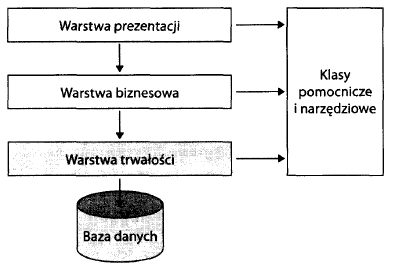
\includegraphics[width=.6\textwidth]{resources/layers.png}
\caption[Warstwowa architektura aplikacji]{Warstwowa architektura aplikacji \cite{hibernate}}
\end{figure}

Zadaniem poszczególnych warstw jest \cite{hibernate}:

\begin{itemize}
\item Warstwa prezentacji -- zawiera logikę interfejsu użytkownika, czyli między innymi kod odpowiedzialny za wyświetlanie okien, formularzy czy też tabel.
\item Warstwa logiki -- jej postać bywa zróżnicowana, przyjmuje się jednak, że powinna zawierać implementację reguł biznesowych i wymagań systemowych, które
zostały uznane za dziedzinę rozwiązywanego problemu.
\item Warstwa trwałości danych -- stanowi grupę klas i komponentów odpowiedzialnych za zapamiętywanie danych i odczytywanie ich z wybranych źródeł. Zawiera ona także
model elementów dziedziny biznesowej.
\end{itemize}

\section{Trwałość danych}

Kluczowym zadaniem podczas tworzenia aplikacji jest zapewnienie trwałości da\-nych, co oznacza zapewnienie, że po zakończeniu działania aplikacji zebrane dane nie mogą
zostać utracone \cite{persistence}. W przeciwnym wypadku znalezienie zastosowania dla takich aplikacji byłoby znacznie cięższym zadaniem a rozwiązanie wielu problemów 
za ich pomocą byłoby niemożliwe. Nie możemy przecież wyobrazić sobie systemu bankowego po którego ponownym uruchomieniu dane na temat wszystkich klientów i
posiadanych przez nich środków zostałyby utracone.

\section{Relacyjne bazy danych}

Większość programistów problem trwałości danych rozwiązuje poprzez wykorzystanie relacyjnych baz danych jako ,,magazynu danych'' oraz języka SQL w roli ,,zarządzającego
danymi''. Pojęcia te są powszechnie znane, jednakże warto przypomnieć ich definicje:

\begin{definition}
Relacyjna baza danych -- zbiór danych w postaci tabel połączonych ze sobą relacjami \cite{rel}.
\end{definition}

\begin{definition}
Język SQL -- strukturalny język zapytań pozwalający na wprowadzanie zmian w strukturze bazy danych, a także zmian w samej bazie czy też pobieranie z niej informacji. Język 
ten opiera się na silniku bazy danych, który pozwala tworzyć zapytania \cite{sql}.
\end{definition}

Duża popularność relacyjnych baz danych wynika z ich licznych zalet, do któ\-rych należą między innymi łatwość modyfikacji przechowywanych w nich danych, zmniejszona
możliwość popełnienia pomyłki czy też duża elastyczność i szybkość w zarządzaniu danymi. Ma to miejsce kosztem zmniejszonej wydajności w stosunku do innych modeli
danych \cite{persistence}. Relacyjne bazy danych swoje zastosowanie znajdują w wielu systemach i platformach technologicznych, są one najczęściej podstawową 
reprezentacją dla elementów biznesowych \cite{hibernate}.

Aby jak najskuteczniej korzystać z narzędzi mapowania obiektowo-relacyjnego warto zaznajomić się z relacyjnymi bazami danych oraz językiem SQL. Wiedza ta umożliwia
tworzenie aplikacji działających sprawniej i bardziej odpornych na wszelkiego rozdzaju błędy. Szczególnie przydatna może okazać się znajomość języka SQL, który jest 
fundamentem mapowania obiektowo-relacyjnego oraz wszystkich innych aplikacji wykorzystujących relacyjne bazy danych w celu zapewnienia trwałości danych.

\section{Programowanie obiektowe}

W aplikacjach stworzonych w oparciu o paradygmat programowania obiektowego, trwałość danych umożliwia przechowanie obiektów po zakończeniu działania aplikacji aż do
momentu kiedy przy jej ponownym uruchomieniu nie zajdzie potrzeba jego wczytania z powrotem. Obiekt jest przechowywany na dysku twardym, a nie jak wcześniej w pamięci
operacyjnej komputera, a ich ilość nie jest ograniczona, ,,utrwalany'' może być pojedyńczy obiekt, ale także całe ich struktury. Warto pamiętać, że większość obiektów nie jest
trwała. Obiekty ulotne mają ograniczony czas życia, związany z tworzonym je procesem czy też metodą \cite{hibernate}.

Obecne relacyjne bazy danych udostępniają zestaw mechanizmów umożliwia\-jących manipulowanie, sortowanie, wyszukiwanie czy też zbieranie danych. Odpo\-wiedzialne są 
one także za nadzorowanie operacjami współbieżnymi  oraz nad inte\-gralnością danych. W przypadku gdy z bazą połączonych jest kilka aplikacji klienckich do jej zadań należy
zarządzanie wszystkimi operacjami oraz unikanie błędów. Decydując się na wykorzystanie relacyjnych baz danych wymienione mechanizmy wykonują sporą część pracy, która
wcześniej musiała zostać wykonana przez pro\-gramistę \cite{persistence}.

\section{Wykorzystanie SQL w C++}

Podczas korzystania z bazy danych w aplikacjach C++ wykorzystywane są łączniki, które przesyłają instrukcje SQL do bazy danych. Instrukcje mogą być tworzone ręcznie lub
generowane przy użyciu kodu C++, zadaniem łącznika jest przesłanie zapytania, odebranie odpowiedzi bazy danych oraz powiadomienie o ewentualnych błędach. 

Większość programistów jednak najbardziej zainteresowana jest problemem biznesowym który musi rozwiązać, a tworzenie zapytań oraz zarządzanie bazą danych im to w pewien
sposób utrudniają. System, który wykona wszystkie zadania zwią\-zane z trwałością danych za programistę tak, żeby ten mógł poświęcić się jedynie rozwiązaniu postawionego
przed nim problemu wydaje się być najlepszym rozwią\-zaniem takiej sytuacji.

W związku z tym, że oprogramowanie dostępu do relacyjnej bazy danych z poziomu obiektowych aplikacji nie należy do najłatwiejszych zadań wiele osób będzie się zastanawiać
czy na prawdę warto to robić. Czy nie lepiej skorzystać z mało popularnych, ale istniejących przecież obiektowych baz danych? Panująca sytuacja pokazuje, że nie. Relacyjne
bazy danych okazują się najbardziej spra\-wdzoną technologią i zdecydowana większość aplikacji je wykorzystuje.

\section{Niedopasowanie paradygmatów}

Jak zauważają autorzy książki ,,Hibernate w akcji'' \cite{hibernate} podstawowym problemem w przypadku wykorzystania relacyjnych baz danych oraz programowania 
obiektowego jest niedopasowanie paradygmatów. Problem ten może zostać podzielony na kilka mniejszych problemów:

\begin{itemize}
\item Problem szczegółowości -- programiści mogą tworzyć nowe klasy z różnym poziomem szczegółowości. Mniej znacząca klasa, na przykład {\tt Adress}, może zostać
osadzona w klasie bardziej znaczącej, na przykład {\tt User}. W bazie danych szczegółowość może zostać zaimplementowana jedynie na po\-ziomie tabeli
{\tt USER} oraz kolumny {\tt ADRESS}. Jest to jednak problem bardzo łatwy do rozwiązania za pomocą tabel powiązanych ze sobą relacjami.
\item Problem podtypów -- dziedziczenie oraz polimorfizm to podstawowe mechanizmy programowania obiektowego i w praktycznie każdej aplikacji znajdziemy ich 
wykorzystanie, relacyjne bazy danych nie udostępniają jednak tych mechanizmów co jest kolejną przyczyną niedopasowania.
\item Problem identyczności -- w przypadku bazy danych encje są identyczne gdy ich klucze główne są takie same. W programowaniu obiektowym obiekty są sobie równe
gdy mają takie same wartości pól lub gdy są identyczne (mają tę samą referencję).
\item Problemy dotyczące asocjacji -- w modelu obiektowym asocjacje reprezentują związki między klasami, na przykład pomiędzy klasami {\tt User} i {\tt Adress}. Języki
obiektowe używają w tym celu referencji czy też wskaźników, stąd też łatwo zauważyć, że asocjacje w modelu obiektowym są kierunkowe lub też dwu\-kierunkowe jeśli
obie klasy mają do siebie referencje. W przypadku baz danych nie istnieją asocjacje dwukierunkowe, wyróżniamy jedynie relacje jeden do wielu oraz jeden do jednego.
Relacja wiele do wielu jest tak na prawdę złożeniem dwóch relacji jeden do wielu z dodatkową tabelą łącznikową, na\-zywaną też asosjacyjną.
\item Problem nawizgacji po grafie obiektów -- sposób dostępu do obiektów zna\-cznie różni się od dosępu do danych w relacyjnych bazach. Chcąc na przykład uzyskać
informacje o ulicy na jakiej mieszka wybrany użytkownik systemu wywołamy metodę {\tt user.getAdress().getStreet()}, wywołanie takie nazywane jest chodzeniem
po grafie obiektu. Przedstawiony sposób niestety nie sprawdza się w przypadku nawigacji w relacyjnych bazach danych. Rozwią\-zaniem jest minimalizacja ilości zapytań
kierowanych do bazy danych, a więc wykorzystanie mechanizmów złączeń jednakże wydajność nigdy nie będzie taka sama jak w przypadku modelu obiektowego.
\end{itemize}

\section{Koszt niedopasowania}

Rozwązanie wymienionych wcześniej problemów dotyczących niedopasowania pa\-radygmatów może okazać się bardzo czasochłonne. Zazwyczaj około 30\% kodu aplikacji
to kod warstwy trwałości danych oraz ręczne generowanie zapytań w celu przechowania danych w bazie. Pomimo tak dużych nakładów pracy, często okazuje się, że
wymagane są liczne poprawki, ponieważ przyjęte rozwiązania okazały się nietrafne.

Największy koszt jest związany z fazą modelowania i trudnościami z dopasowaniem dobrze znanego programistom modelu obiektowego do niekiedy trudniejszego do zrozumienia
modelu relacyjnego. Problem ten udaje się często ro\-związać kosztem zalet modelu obiektowego takich jak niewykorzystanie dziedziczenia czy polimorfizmu. Problem niedopasowania
modeli prowadzi do niskej elastyczności i utraty produktywności tworzonych aplikacji, co prowadzi w ostateczności ku wyższym kosztom tworzenia oprogramowania \cite{hibernate}. 

\section{Mapowanie obiektowo-relacyjne}

Poza przedstawionym wcześniej klasycznym podejściem zapewniania trwałości da\-nych w aplikacjach, w którym programista sam tworzy bazę danych a potem nią zarządza
konstruując zapytania w języku SQL, istnieje także inne rozwiązanie tego problemu nazywane najczęściej mapowaniem, bądź też odwzorowaniem obiektowo-relacyjnym 
\cite{hibernate}.

W pierwszym rozdziale podczas opisu problematyki pracy została przedstawiona uproszczona definicja mapowania obiektowo-relacyjnego, biorąc pod uwagę pojęcia opisane
w tym rozdziale można ją tym razem zapisać w sposób następujący:

\begin{definition}
Mapowanie obiektowo-relacyjne --  automatyczna i niewidoczna dla uży\-tkownika realizacja trwałości obiektów w aplikacji zamieniająca je na wpisy w relacyjnej bazie danych
na podstawie metadanych opisujących klasę. Mapowanie działa jako dwukierunkowy translator danych z jednej reprezentacji w inną \cite{hibernate}. 
\end{definition}

\begin{figure}[h]
\centering
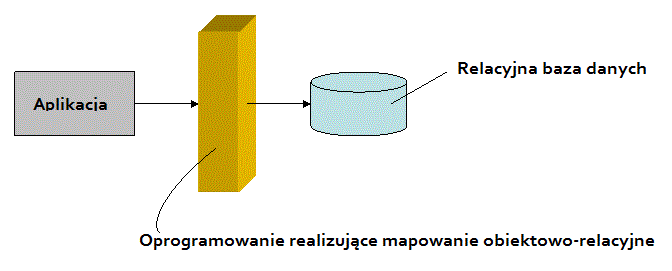
\includegraphics[width=.9\textwidth]{resources/orm.png}
\caption{Mapowanie obiektowo-relacyjne}
\end{figure}

Narzędzia realizujące mapowanie obiektowo-relacyjne składają się z w wię\-kszości przypadków następujących elementów \cite{hibernate}:

\begin{itemize}
\item Interfejsu do przeprowadzania podstawowych operacji CRUD\footnote{~utwórz, odczytaj, zaktualizuj oraz usuń (ang. Create, Read, Update and Delete)} na obiektach
klas zapewniających trwałość.
\item Interfejsu umożliwiającego tworzenie zapytań związanych z klasami oraz ich właściwościami.
\item Narzędzia do określania metadanych.
\item Technik takiej implementacji mapowania, aby poprawnie współgrało ono z obiektami transakcyjnymi wykonując wszystkie dostępne operacje. 
\end{itemize}

W zasadzie więc terminu mapowania obiektowo-relacyjnego można użyć w odniesieniu do dowolnej warswy trwałości, która zapytania do bazy danych generuje automatycznie
na podstawie opisu w postaci metadanych. Tworzenie jednak takiego generatora dla pojedyńczej aplikacji często mija się z celem i lepszym rozwiązaniem jest skorzystanie z
gotowego narzędzia służacego do mapowania bądź też własnoręczna implementacja warstwy trwałości w wybranej aplikacji. W przypadku wyboru jednego z gotowych narzędzi
w ogóle nie musimy zajmować się implementacją warstwy trwałości, ponieważ korzystamy z już wcześniej przygotowanej.

Do sposobów implementacji mapowania obiektowo-relacyjnego należą \cite{hibernate}:

\begin{itemize}
\item Pełna relacyjność -- cała aplikacja, włączając w to interfejs użytkownika, zaprojektowana jest wokół modelu relacyjnego i podstawowych operacji języka SQL. Aplikacje
takie część logiki mogą mieć przeniesione do warstwy bazy danych.
\item Lekkie odwzorowanie obiektów -- encje są reprezentowane przez ręczne na\-pisane klasy odpowiadające tabelom relacynym. Kod SQL zostaje schowany przed logiką
aplikacji dzięki wzorcom projektowym.
\item Średnie odwzorowanie obiektów -- aplikacja jest zaprojektowana wokół modelu obiektowego. Kod SQL jest generowany dynamicznie przez szkielet systemu.
\item Pełne odwzorowanie obiektów -- obsługuje wyrafinowane modele obiektowe stosując kompozycję, dziedziczenie i polimorfizm. Warstwa trwałości w spo\-sób niewidoczny
implementuje zapis i odczyt danych. Ten poziom funkcjonalności jest najtrudniejszy do osiągnięcia i uzyskiwanie go na potrzeby pojedyńczej aplikacji nie ma sensu.
\end{itemize}

Dlaczego warto korzystać z mapowania obiektowo-relacyjnego? Podstawową zaletą dla programisty jest z pewnością możliwość uniknięcia pisania własnoręcznie wszystkich
zapytań, a zamiast tego skorzystanie z gotowych metod wybranego narzędzia. Mogłoby to sugerować, że decydując się na korzystanie z mapowania nie musimy znać się
ani na relacyjnych bazach danych, ani na języku SQL, jest to jednak nieprawda, ponieważ wydajność tworzonych w taki sposób aplikacji byłaby znacznie mniejsza od tych
napisanych przez programistów którym te pojęcia nie są obce. Przyjrzyjmy się jeszcze raz podstawowym zaletom mapowania obiektowo-relacyjnego \cite{hibernate}:

\begin{itemize}
\item Produktywność -- warstwa trwałości jest bardzo niewdzęczną warstwą do oprogramowania, decydując się na skorzystanie z narzędzi mapujących problem ten zostaje
wyeliminowany a cała uwaga programisty może zostać poświę\-cona innym warstwom aplikacji.
\item Konserwacja -- brak warstwy logiki w kodzie napisanym przez programistę czyni system bardziej zrozumiałym, czytelniejszym, a co za tym idzie łatwie\-jszym do 
przekształcenia.
\item Wydajność -- prawdą jest stwierdzenie, że warstwa trwałości napisana ręcznie przez programistę potrafi być co najmniej tak szybka jak ta wygenerowana automatycznie.
Podobnie prawdą jest, że dowolny program napisany w C++ można napisać w Assemblerze by działał co najmniej tak szybko jak ten pierwszy. Jednak jak dobrze wiadomo,
znacznie trudniejszym zadaniem jest napisanie programu w języku asemblera aby działał on tak samo sprawnie jak ten napisany w C++. Aby to zrobić trzeba bardzo dobrze
znać Assemblera, analogiczna sytuacja ma miejsce podczas własnoręcznego tworzenia warstwy trwałości i znajomości języka SQL.
\item Niezależność -- abstrakcja języka SQL uwalnia programistę od jego szczegółów i różnych jego dialektów w poszczególnych systemach bazodanowych. Większość narzędzi
obsługuje wiele systemów bazodanowych, a więc nawet ich zmiana po napisaniu aplikacji nie powinna być problemem.
\end{itemize}

Mapowanie obiektowo-relacyjne jest rozwiązaniem sprawdzającym się obecnie w bardzo dużej ilości istniejących już aplikacji i jego wybór przed własnoręczną implementacją 
zapytań jest najczęściej trafną decyzją. W chwili są to dwa najpopularniejsze rozwiązania, przy czym mapowanie jest obecnie najczęściej wybierane w związku z
niedopasowaniem obiektowo-relacyjnym.

\section{Aplikacje szkieletowe}

Na wstępie aplikacje szkieletowe zostały opisane jako ,,fundamenty'' dla tworzonych przez programistów aplikacji, warto przypomnieć tutaj dokładniejszą definicję tego
pojęcia:

\begin{definition}
Aplikacja szkieletowa\footnote{~ang. Framework} -- szkielet budowy aplikacji. Definiuje strukturę aplikacji oraz jej ogólny mechanizm działania, dostarcza zestaw komponentów
i bibliotek ogólnego przeznaczenia do wykonywania określonych zadań \cite{framework}.
\end{definition}

Charakterystycznymi cechami aplikacji szkieletowych są między innymi \cite{framework}:

\begin{itemize}
\item Gotowy szkielet dla tworzonych aplikacji.
\item Narzucony przepły sterowania.
\item Domyślna konfiguracja.
\item Komponenty do rozbudowy.
\end{itemize}

Do zalet aplikacji szkieletowych można zaliczyć \cite{framework}:

\begin{itemize}
\item Szybka realizacja projektu -- część kodu jest gotowa, a więc oszczędzamy sporo czasu potrzebnego na jego napisanie.
\item Poprawa jakości kodu oraz większa niezawodność -- gotowy kod został wielokrotnie przetestowany oraz był używany przez wielu innych programistów, a więc jeśli coś
nie działa to w większości przypadków wina błędu użytkownika.
\item Wsparcie twórców frameworka -- jeśli jednak uda nam się znaleźć jakiś błąd, zawsze możemy liczyć na wsparcie ze strony twórców oprogramowania.
\end{itemize}

Do ich wad natomiast zaliczamy \cite{framework}:

\begin{itemize}
\item Złożoność -- zakres działań aplikacji szkieletowych jest bardzo szeroki, a co za tym idzie ich sposób działania nie jest zawsze oczywisty.
\item Koszt szkoleń -- aby poradzić sobie ze złożonością, najlepszym wyjściem jest poświęcenie dodatkowego czasu na szkolenie w zakresie wybranego oprogramowania.
\item Zredukowana wydajność -- w bardziej skomplikowanych systemach wykorzystanie aplikacji szkieletowych może mieć wspłw na spadek wydajności systemu, dzieje się
tak w związku z niedopasowaniem wybranej aplikacji do systemu.
\end{itemize}

\chapter[Analiza istniejących rozwiązań]{Analiza istniejących rozwiązań mapowania obiektowo-relacyjnego w języku C++} \label{analiza}

\section{Kryteria analizy}

W pierwszym rozdziale niniejszej pracy pojawiła się informacja, że istnieją już biblioteki oraz aplikacje szkieletowe realizujące mapowanie obiektowo-relacyjne w języku C++,
jednakże jest ich mniej niż w przypadku innych znanych języków programowania. W tym rozdziale zostanie przeprowadzona ich dokładniejsza analiza, do której potrzebne
jest wskazanie kryteriów, które zostaną przeanalizowane. Pod uwagę zostałe wzięte następujące aspekty:

\begin{itemize}
\item Charakter oprogramowania -- przede wszystkim istotny jest fakt, czy wybrane narzędzie należy do tak zwanego ,,wolnego oprogramowania''\footnote{~ang. open-source
software}, a co za tym idzie czy jego użytkownik może podejrzeć i w razie potrzeby zmodyfikować jego kod źródłowy oraz podzielić się wprowadzonymi przez siebie zmianami z innymi 
jego użytkownikami. W tensposób oprogramowanie ulega ciągłemu rozwojowi, a jego działanie łatwiej zrozumieć.
\item Licencja -- wielce istotny jest fakt czy wybrane oprogramowanie jest darmowe oraz na jakich zasadach może zostać wykorzystywane. Mało restrykcyjna licencja jest z
pewnością zaletą.
\item Wspierane systemy zarządzania bazą danych -- tutaj zasada jest prosta, im więcej rodzajów baz danych jest wspieranych tym lepiej. Dużą zaletą jest także rozszerzalność
orpgoramowania, czyli możliwość dodania wsparcia dla wybranych baz samodzielnie.
\item Wykorzystywane biblioteki i aplikacje szkieletowe -- część narzędzi wykorzystuje inne, takie jak aplikacja szkieletowa Qt czy bibliotekę boost. Istotne jest to czy użytkownik
też musi wykorzystywać dane rozwiązania w swojej aplikacji.
\item Poziom skomplikowania interfejsu -- konieczność wywoływania sekwencji wielu metod w celu wykonania podstawowych operacji w bazie danych czy też w celu połączenia
się z nią nie należy z pewnością do zalet oprogramowania.
\item Dostępność generatora opisu -- generator opisu jest w stanie znacznie uprościć wykorzystanie narzędzi mapowania obiektowo-relacyjnego, więc jego obecność jest
dodatkową zaletą.
\item Dodatkowe możliwości -- wiele narzędzi posiada specyficzne dla siebie zalety, w tym punkcie zostaną one wyszczególnione.
\end{itemize}

\section{Porównanie istniejących rozwiązań}

\subsection{Biblioteka QxOrm}

Analizę rozpoczyna najpopularniejsza biblioteka realizujaca mapowanie obiektowo-relacyjne w języku C++, czyli QxOrm.

\begin{figure}[h]
\centering

\includegraphics[width=.5\textwidth]{resources/qxorm.png}
\caption[Biblioteka QxOrm]{Biblioteka QxOrm \cite{qxorm}}
\end{figure}

\newpage

Analizę wyznaczonych kryteriów przedstawia poniższa tabela:

\begin{table}[h]
\centering
\begin{tabular}{| l | l |} 
\hline 
Charakter oprogramowania & open-source \\ \hline
Licencja & GNU/GPL  \\ \hline
Wspierane bazy danych & MySQL, PostgreSQL, Oracle, \\ \hline
& SQLite, IBM DB2, InterBase, SysBase \\ \hline
Wykorzystywane narzędzia & Qt, boost  \\ \hline
Poziom skomplikowania interfejsu & wysoki  \\ \hline
Dostępność generatora opisu & tak  \\ \hline
Dodatkowe możliwości &  edytor encji, walidacja danych,   \\ \hline
& serializacja danych, pamięć cache  \\ \hline
\end{tabular} 
\caption{Analiza biblioteki QxOrm}
\end{table}

Konfiguracja QxOrm jest dość rozbudowana, a co za tym idzie skomplikowana. Rejestracja klas wymaga używanie wielu funkcji i makr w pliku nagłówkowym \cite{qxorm}:

\lstinputlisting[style=customc,caption=Przykładowy plik nagłówkowy klasy korzystającej z QxOrm]{resources/qxorm_sampleclass.h}

A także w pliku klasy \cite{qxorm}:

\lstinputlisting[style=customc,caption=Przykładowy plik klasy korzystającej z QxOrm]{resources/qxorm_sampleclass.cpp}

Samo wykorzystanie QxOrm także nie należy do najłatwiejszych zadań, istotne jest poprawne skonfigurowanie bazy danych z poziomu kodu, oraz wykonanie odpowiednich
sekwencji metod \cite{qxorm}:

\lstinputlisting[style=customc,caption=Przykładowy plik klasy korzystającej z QxOrm]{resources/qxorm_sample.cpp}

\subsection{Biblioteka Debea}

Kolejnym narzędziem poddanym analizie została biblioteka Debea:

\begin{figure}[h]
\centering

\includegraphics[width=.5\textwidth]{resources/debea.jpg}
\caption[Biblioteka Debea]{Biblioteka Debea \cite{debea}}
\end{figure}

Analizę wyznaczonych kryteriów przedstawia poniższa tabela:

\begin{table}[h]
\centering
\begin{tabular}{| l | l |} 
\hline 
Charakter oprogramowania & open-source \\ \hline
Licencja & wxWindows  \\ \hline
Wspierane bazy danych & MySQL, IBM DB2, Oracle, MSSQL\\ \hline
Wykorzystywane narzędzia & brak  \\ \hline
Poziom skomplikowania interfejsu & wysoki  \\ \hline
Dostępność generatora opisu & tak  \\ \hline
Dodatkowe możliwości &  serializacja danych  \\ \hline
\end{tabular} 
\caption{Analiza biblioteki Debea}
\end{table}

Konfiguracja Debei jest stosunkowo prosta, odbywa się z poziomu kodu. Wykonywanie podstawowych operacji nie należy jednak do najprostszych, oto przykładowe połączenie
z bazą danych i wykonanie na niej podstawowych operacji z użyciem Debei:

\lstinputlisting[style=customc,caption=Przykładowy użycie Debei]{resources/debea_sample.cpp}

Treść licencji bibliotek wxWindows można znaleźć pod adresem {\tt http://open\-source.org/licenses/wxwindows.php}.

\chapter{Aplikacja szkieletowa Qubic} \label{qubic}

\section{Moduły tworzonej aplikacji}

W rozdziale pierwszym w skrócie został przedstawiony schemat współpracy modułu tworzonego przez autora tej pracy a autora pracy, której tematem jest ,,Generator opis
mapowania obiektowo-relacyjnego w języku C++''. W tym podrozdziale opis ten zostanie rozwinięty.

Chcąc w jak największym stopniu zautomatyzować obsługę połączenia z bazą oraz zminimalizować czas jaki programista będzie musiał poświęcić na oprogra\-mowywanie
komunikacji pomiędzy programem a bazą danych zdecydowaliśmy się na wprowadzenie generatora opisu, który tę część pracy wykona za użytkownika Qubica.

Zadaniem generatora jest wygenerowanie plików klas, plików nagłówkowych oraz pliku projektu Qt w oparciu o istniejącą bazę danych. Moduł tworzony przez autora niniejszej
pracy będzie wykorzystywany w wygenerowanym kodzie, a także w kodzie napisanym przez użytkownika Qubica. W momencie zakończenia pracy generatora wygenerowana
aplikacja będzie w pełni gotowa do przechowywania danych z bazie bez konieczności tworzenia zapytań. W celu przechowania obiektów aplikacji, ich modifikacji, załadowania 
czy usunięcia z bazy danych wystarczy uruchomienie odpowiednich metod Qubica.

Dalsza część tego rozdziału została poświęcona w zdecydowanej większości modułowi Qubica zajmującego się mapowaniem obiektowo-relacyjnym.

\section{Analiza wymagań}

\subsection{Wymagania funkcjonalne}

Podczas projektowania Qubica przyjęto następujące założenia w celu jak najlepszego odwzorowania cech mapowania obiektowo-relacyjnego:

\begin{itemize}
\item Aplikacja musi umożliwiać podstawowe operacje mapowania obiektowo-rela\-cyjnego, a więc zapisywanie obiektów do bazy danych, ich odczyt, aktualizowanie obiektów
już zapsanych w bazie oraz ich usuwanie.
\item Aplikacja musi udostępniać interfejs do tworzenia zapytań z poziomu kodu, dzięki temu jej użytkownik nie musi znać języka SQL.
\item Aplikacja musi udostępniać funkcje dostępu do powiązanych danych w przypadku wystąpienia relacji różnych od jeden do jednego. Użytkownik powinien mieć możliwość
uzyskania dostępu do obiektów powiązanych z wybranym obiektem bez konieczności własnoręcznego konstruowania zapytań.
\item Aplikacja powinna posiadać wsparcie dla wielu rodzajów baz danych, ewentualnie musi być ona łatwo rozszerzalna.
\item Aplikacja musi posiadać możliwość wykorzystania transakcji.
\item Aplikacja musi posiadać możliwość konfiguracji.
\end{itemize}

\subsection{Wymagania niefunkcjonalne}

Do wymagań niefunkcjonalnych postawionych projektowanej aplikacji należą:

\begin{itemize}
\item Użytkowanie aplikacji powinno być jak najbardziej intuicyjne, co za tym idzie kod użytkownika mający za zadanie wykonywać podstawowe operacje powinien zajmować
jak najmniej linii.
\item Aplikacja musi działać możliwie szybko, czas podstawowych operacji nie powinien znacząco odbiegać od tego w przypadku gdy użytkownik sam two\-rzyłby zapytania do bazy.
\item Aplikacja musi rozpoznawać relacje jeden do jednego, jeden do wielu oraz wiele do wielu i odpowiednio je obsługiwać.
\item Pamięć w trakcie działania aplikacji musi być odpowiednio zarządzana, niedopuszczalne są żadne wycieki pamięci czy też zapętlenia się programu.
\item Błędy pojawiające się w trakcie działania aplikacji powinny być prawidłowo obsługiwane i sygnalizowane użytkownikowi.
\end{itemize}

\section{Projekt}

\subsection{Rodzaj aplikacji}

\begin{figure}[h]
\centering

\includegraphics[width=.55\textwidth]{resources/qb.png}
\caption{Logo tworzonej aplikacji szkieletowej}
\end{figure}

Qubic jest aplikacją szkieletową, czyli strukturą do wykorzystywaną do budowy innych aplikacji. Jego podstawowym zadaniem jest realizacja mapowania obiektowo-relacyjnego,
czyli udostępnienie funkcjonalności pozwalającej na przechowywanie obiektów w bazie danych.

W celu stworzenia aplikacji w oparciu o Qubica użytkownik musi przygotować bazę danych na podstawie której wygenerowany zostanie plik projektu Qt wraz z plikami nagłówkowymi
oraz plikami klas. W tym momencie aplikacja posiada już oprogramowany dostęp do danych i użytkownik może zająć się implementowaniem własnej logiki czy też warstwy widoku.

\subsection{Diagram klas}

Diagram klas Qubica przedstawia rysunek \ref{diagram}:

\newpage
\noindent
\begin{minipage}{\linewidth}
\makebox[\linewidth]{
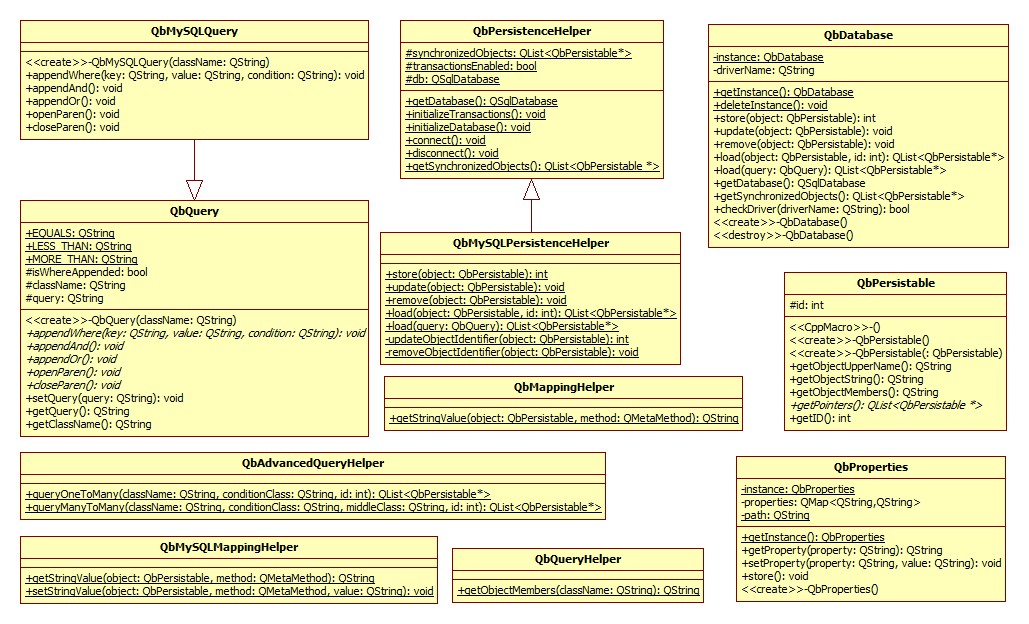
\includegraphics[keepaspectratio=true, width=.9\textwidth]{resources/diagram.jpeg}}
\captionof{figure}{Diagram klas}
\label{diagram}
\end{minipage}

\subsection{Wzorce projektowe}

Jednym z wzorców projektowych, które znalazły zastosowanie w Qubicu jest Singleton. Do jego największych zalet należy fakt, że klasa go wykorzystująca może posiadać 
co najwyżej jedną instancję do której istnieje globalny dostęp. Singleton swoje zastosowanie znajduje w przypadku gdy programista chce ograniczyć liczbę instancji dla 
wybranych klas a także samemu odpowiadać za ich tworzenie. W przypadku Qubica został on wykorzystany w klasach {\tt QbDatabase} oraz {\tt QbProperties}. Tworzenie 
więcej niż jednej instancji tych klas nie ma sensu biorąc pod uwagę specyfikę projektu, więc najlepszym rozwiązaniem wydaje się być zablokowanie tej możliwości użytkownikowi. 

\subsection{Środowisko programistyczne}

Qubic został napisany w języku C++ w oparciu o aplikację szkieletową Qt, co za tym idzie wybór platformy należy do użytkownika i równie dobrze może to być Windows jak i Linux.
Zarówno wybór bazy danych nie został narzucony z góry, co prawda na potrzeby projektu zaimplementowana została obsługa tylko dla bazy MySQL jednak zapewniona została 
łatwa rozszerzalność i dodanie obsługi dla innych rodzajów baz danych nie powinna być problemem.

Jedyną biblioteką wykorzystywaną przez Qubica jest QsLog \cite{qslog} odpowiedzialny za logowanie wydarzeń w konsoli Qt. Jest to bardzo przydatna funkcja, która umożliwia
szybkie zlokalizowanie pojawiających się problemów.

\subsection{System kontroli wersji}

Podczas pracy nad projektami w których bierze udział więcej niż jedna osoba bardzo dobrym rozwiązaniem jest korzystanie z systemów kontroli wersji. Ułatwiają one wspólną
pracę oraz organizację tworzonych projektów.

Wybór autorów Qubica padł na dobrze znany serwis GitHub \cite{github}. Poza repozytorium na którym znaleźć można kod źródłowy Qubica podczas implementacji projektu
wykorzystany został system Issues and Milestones\footnote{~problemy oraz kamienie miliowe}, który ułatwia organizację pracy nad projektem.

\begin{figure}[h]
\centering
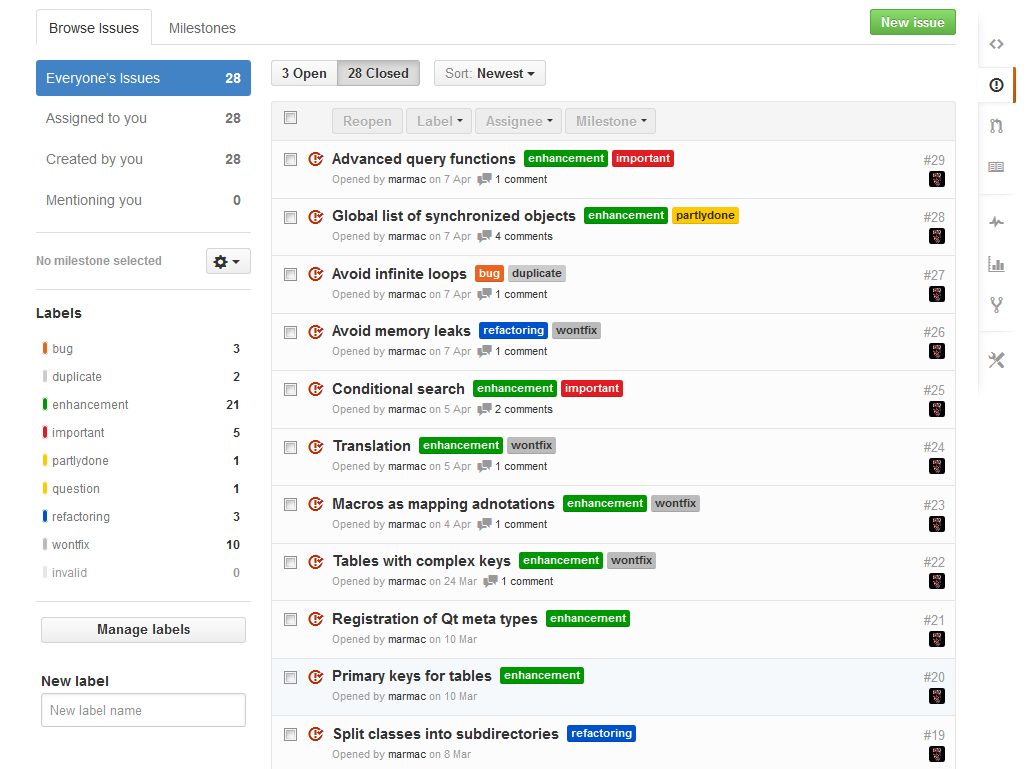
\includegraphics[width=\textwidth]{resources/githubissue.png}
\caption{Przejrzysty widok systemu GitHub Issues}
\end{figure}

\begin{figure}[h!]
\centering
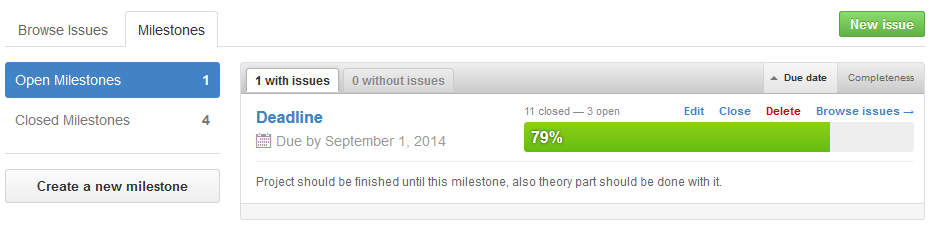
\includegraphics[width=\textwidth]{resources/githubmilestone.png}
\caption{Przejrzysty widok systemu GitHub Miletsones}
\end{figure}

\section{Implementacja}

\subsection{Połączenie z bazą danych}

Obsługa połączenia z bazą danych należy do fundamentalnych operacji realizowanych przez narzędzia zajmujące się mapowaniem obiektowo-relacyjnym, nie inaczej jest w
przypadku Qubica. W związku z tym, że w innych analizowanych narzędziach można było się napotkać na uciążliwą konfigurację odbywającą się głównie z poziomu kodu
Qubic korzysta z pliku konfiguracyjnego, który przechowywuje całą jego konfigurację. Ponadto sama obsługa połączenia jest niewidoczna dla użytkownika, ponieważ
połączenie nawiązywane jest podczas uzyskania dostępu do instancji {\tt Singleton}. 

\subsection{Interfejs CRUD}

Kluczowym modułem narzędzi programistycznych realizujących mapowanie obiekt\-owo-relacyjne jest interfejs CRUD umożliwiający manipulowanie danymi w bazie danych z 
poziomu kodu. Interfejs ten dostępny jest w podstaci co najmniej czterech metod, które jako argumenty przyjmują obiekty dziedziczące po jednej z klas Qubica -- 
{\tt QbPersistable}. Umożliwia to wykorzystanie polimorfizmu, a przecież podczas operacji na obiektach od samego początku nie znany jest dokładny typ obiektu.

Aby mapowanie mogło skutecznie działać potrzebny jest jego jednoznaczny opis, część narzędzi je realizujących korzysta z adnotacji, które określają mapowanie pomiędzy
konkretnymi polami klas a konkretnymi tabelami w bazie danych. W Qubicu problem ten został rozwiązany w trochę inny sposób, który umożliwia stworzony generator opisu
mapowania obiektowo-relacyjnego. Generowane pliki klas są tworzone według ściśle określonych zasad, co oznacza, że nazwy metod dostępowych odpowiadają w pewien
sposób nazwom tabel i ich kolumn. Przykładowo dla kolumny o nazwie {\tt NAME} w tabeli {\tt EMPLOYEE} w pliku klasy {\tt Employee} zostaną wygenerowane metody 
{\tt getName()} oraz {\tt setName(QString name)}. Wie\-dza ta została wykorzystana w trakcie korzystania z mechanizmu refleksji. Konfiguracja samego mapowania nazw
została zapisana w pliku konfiguracyjnym Qubica.

Schematy działania czterech podstawowych metod dostępu przedstawiają po\-niższe schematy blokowe:

\newpage
\begin{figure}[H]
\centering
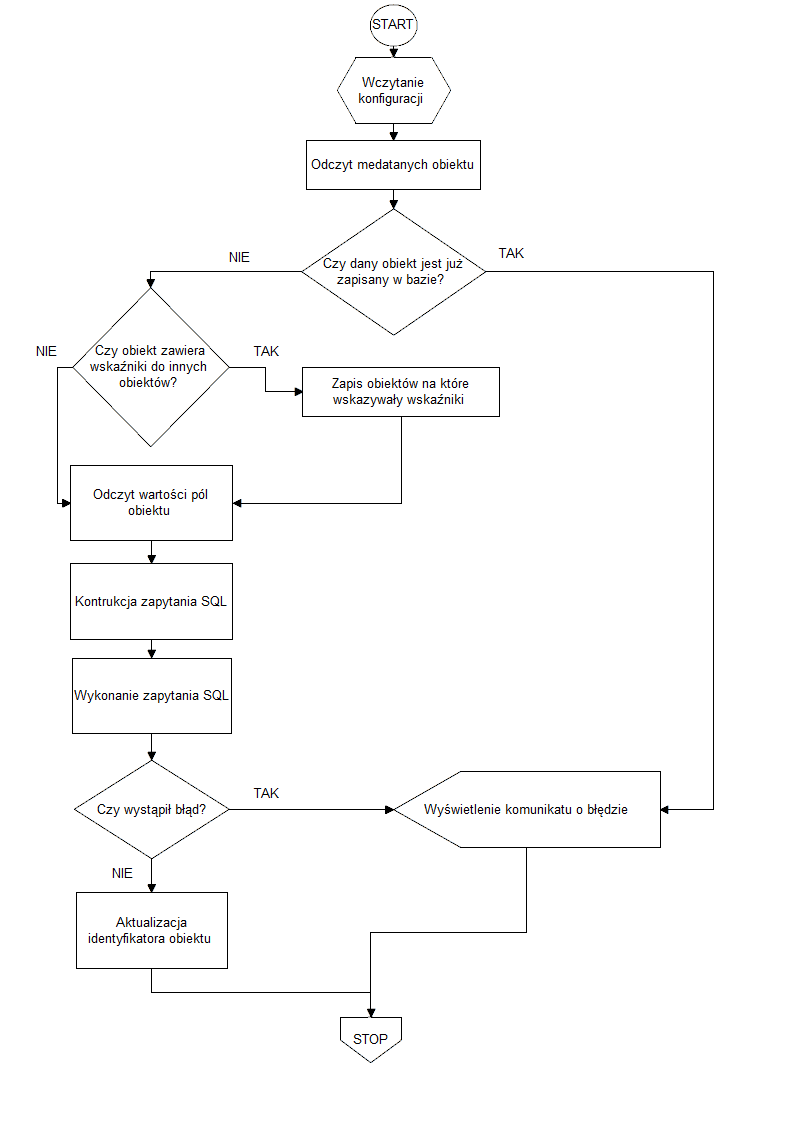
\includegraphics[width=\textwidth]{resources/store_schema.png}
\caption{Schemat blokowy metody zapisującej obiekty w bazie danych}
\end{figure}

\begin{figure}[H]
\centering
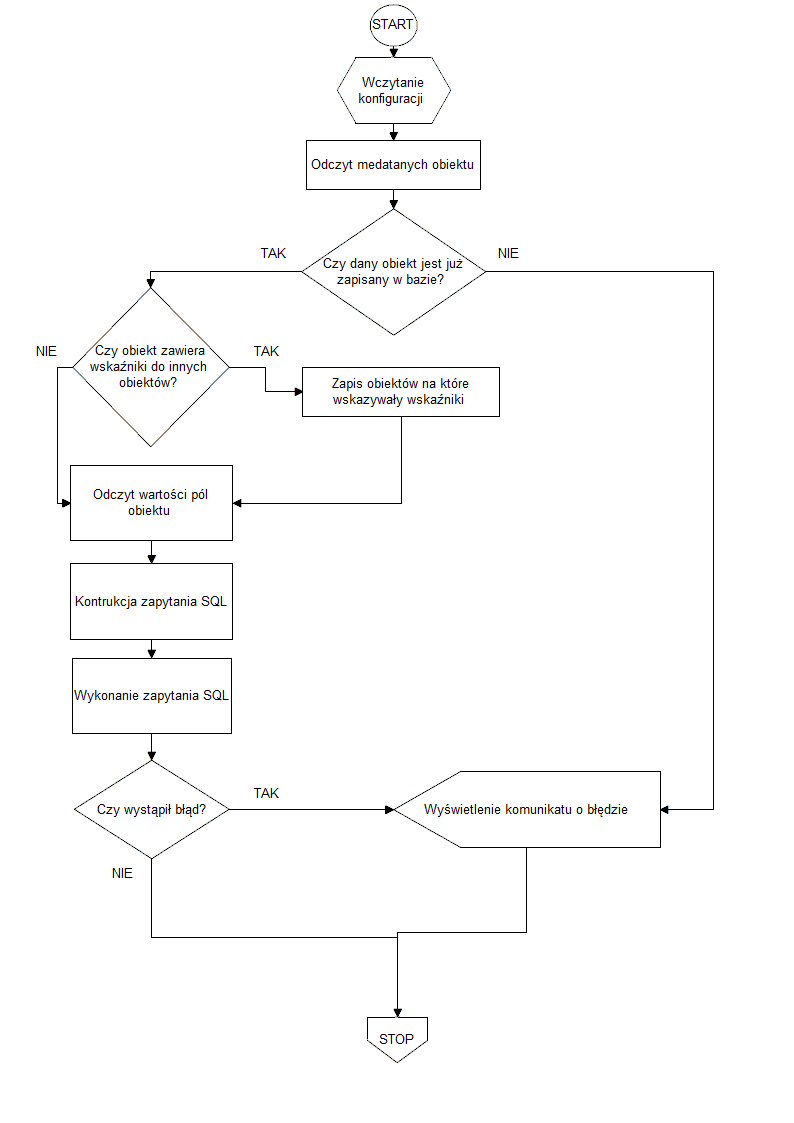
\includegraphics[width=\textwidth]{resources/update_schema.png}
\caption{Schemat blokowy metody aktualizującej obiekty w bazie danych}
\end{figure}

\begin{figure}[H]
\centering
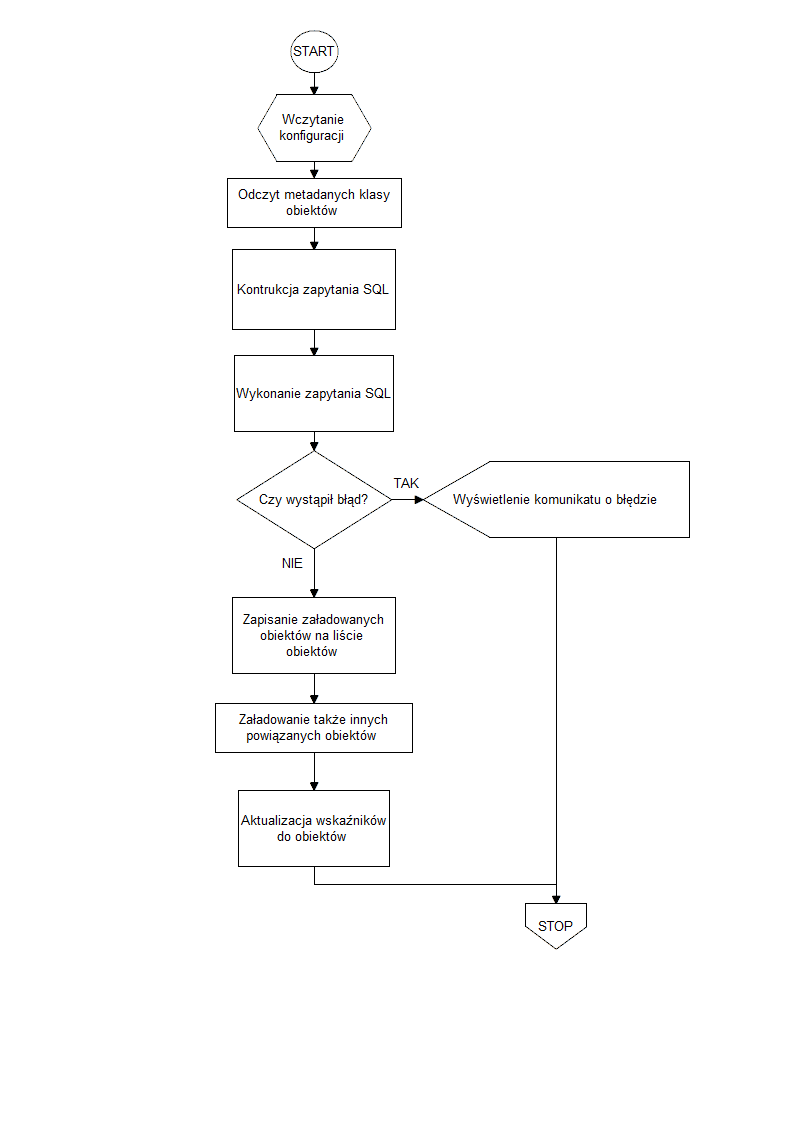
\includegraphics[width=\textwidth]{resources/load_schema.png}
\caption{Schemat blokowy metody ładującej obiekty z bazy danych}
\end{figure}

\begin{figure}[H]
\centering
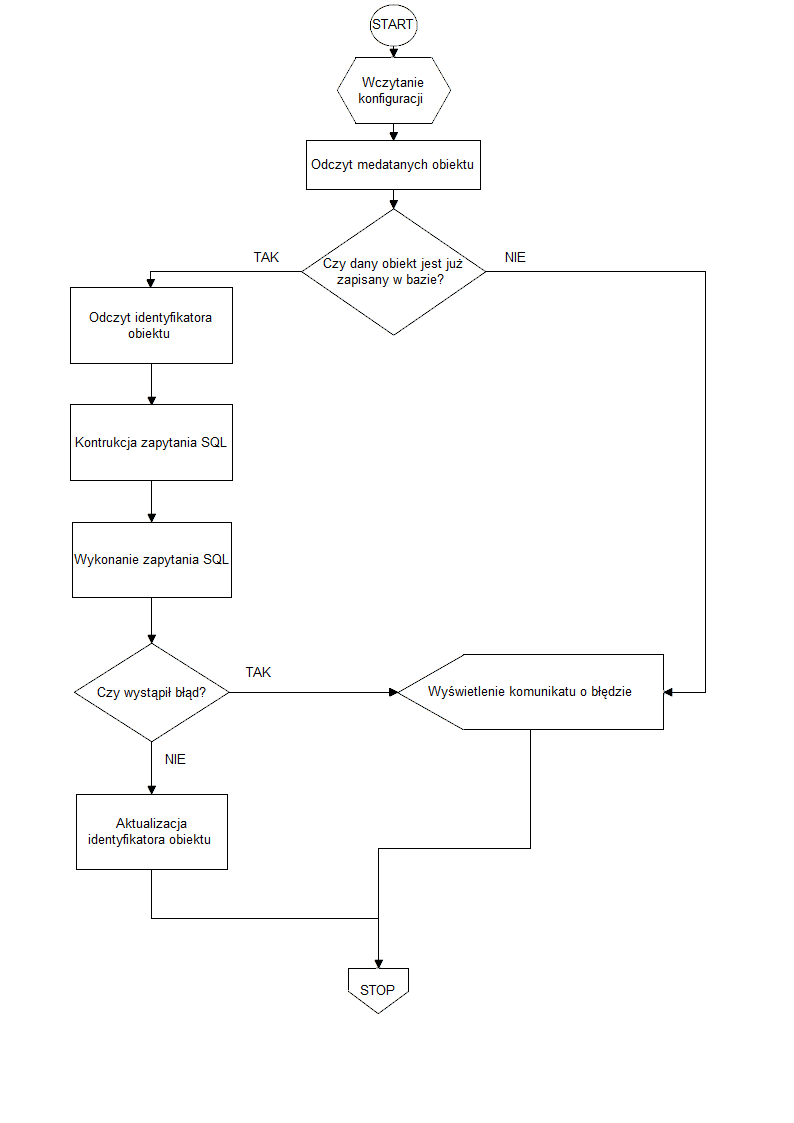
\includegraphics[width=\textwidth]{resources/remove_schema.png}
\caption{Schemat blokowy metody usuwającej obiekty z bazy danych}
\end{figure}

\newpage

\subsection{Interfejs do tworzenia zapytań}

Interfejs ten został utworzony w celu ujednolicenia zapytań jakie mogą być przesyłane do różnego rodzaju baz danych. Użytkownik za jego pomocą może skonstruować
obiekt zapytania, który to w momencie przesłania do bazy danych jest przetłumaczony na dialekt języka SQL z którego aktualnie użytkownik korzysta. Przykład wykorzystania
takiego interfejsu może wyglądać następująco:

\lstinputlisting[style=customc,caption=Tworzenie zapytań Qubica]{resources/sample_query.cpp}

\subsection{Metody dostępu do powiązanych danych}

Charakterystycznymi elementami relacyjnych baz danych są relacje jeden do wielu oraz wiele do wielu, składające się tak na prawdę z tabeli łącznikowej oraz dwóch relacji
jeden do wielu. Dużym usprawnieniem dla aplikacji jest możliwość uzyskania obiektów powiązanych z wybranym obiektem, Qubic udostępnia taką możliwość.

Weźmy pod uwagę dwie klasy obiektów {\tt Employee} oraz {\tt Company}. W modelu relacyjnym tabela {\tt EMPLOYEE} zawiera odwołanie do tabeli {\tt COMPANY} dzięki
czemu posiadamy informacje dla jakiej firmy pracuje wybrany pracownik, w modelu obiektowym zrealizowane to jest za pomocą referencji lub też wskaźników. Co jednak jeśli
potrzebujemy informacji o wszystkich pracownikach danej firmy? Ani obiekt ani encja w tabeli nie posiada takich informacji, na pomoc przychodzą wygenerowane przez
generator opisu tzw. metody dostępu do powiązanych danych. W przedstawionym przypadku jest to metoda {\tt getEmployees}, którą możemy wywołać na dowolnym obiekcie
klasy {\tt Company}.

\section{Przykładowa aplikacja wykorzystująca Qubica}

W celu zaprezentowania sposobu działania Qubica rozważmy następujący schemat bazy danych, której struktura zawiera zarówno relację jeden do wielu jak i wiele do wielu:

\lstinputlisting[style=customsql,caption=Plik tworzący przykładową bazę danych]{resources/sample_db.sql}

Na podstawie zaprezentowanego schematu wygenerowane zostały pliki klas oraz projektu, następnie w celach prezentacyjnych stworzony został zaprezentowany poniżej
plik, który wykonuje podstawowe operacje na bazie danych:

\newpage

\lstinputlisting[style=customc,caption=Plik przedstawiający przykładową aplikację korzystającą z Qubica]{resources/sample_app.cpp}

Jak widać wykonanie podstawowych operacji CRUD ogranicza się do wywołania pojedyńczej funkcji, bez konieczności wcześniejszego zapewnienia połączenia z bazą ani
konfiguracji z poziomu kodu. Jest to bardzo dobry wynik biorąc pod uwagę poprawne działanie aplikacji widoczne na kolejnym listingu, tym razem jest to zrzut z konsolii
wykonanego programu, przy użyciu świeżo utworzonej bazy danych:

\lstinputlisting[style=customcmd,caption=Plik wynikowy przykładowej aplikacji korzystającej z Qubica]{resources/sample_cmd.txt}

Dodatkowo rezultatem pracy programu był szczegółowy log Qubica, jednakże ze względu na jego długość został on pominięty w niniejszej pracy. Wszystkie operacje zostały
wykonane zgodnie z oczekiwaniami, co pozwala sądzić, że mapowanie obiektowo-relacyjne co najmniej w tym kontekście odbywa się poprawnie.

\section{Analiza Qubica}

W rozdziale trzecim przedstawiona została analiza istniejących narzędzi służących do mapowania obiektowo-relacyjnego w języku C++, między innymi na jej podstawie
stworzona została aplikacja szkieletowa Qubic realizująca to samo zagadnienie. Jej analiza wygląda następująco:

\begin{table}[h]
\centering
\begin{tabular}{| l | l |} 
\hline 
Charakter oprogramowania & open-source \\ \hline
Licencja & GNU/GPL  \\ \hline
Wspierane bazy danych & MySQL oraz łatwa możliwość \\ \hline
&  rozszerzenia o inne rodzaje baz \\ \hline
Wykorzystywane narzędzia & Qt  \\ \hline
Poziom skomplikowania interfejsu & niski  \\ \hline
Dostępność generatora opisu & tak  \\ \hline
Dodatkowe możliwości &  walidacja danych, metody dostępu  \\ \hline
& do powiązanych obiektów \\ \hline
\end{tabular} 
\caption{Analiza aplikacji szkieletowej Qubic}
\end{table}

W porównaniu do przeanalizowanych wcześniej narzędzi Qubic wyróżnia się przede wszystkim niskim poziomem skomplikowania interfejsu, co można zauważyć szczególnie w
poprzedniej sekcji opisującej przykładową aplikacje stworzoną w oparciu o Qubica. Ponadto, udostępnia on wszystkie podstawowe mechanizmy charakterystyczne dla mapowania
obiektowo-relacyjnego, a także walidację danych podzczas generowania opisu czy gotowe metody dostępu do obiektów powiązanych. 

Qubic należy do wolnego oprogramowania udostępnianego na licencji GNU/GPL podobnie jak i większość analizowanych narzędzi. Istotną jego cechą jest wykorzystanie aplikacji
szkieletowej Qt, podobnie jak analizowana wcześniej biblioteka QxOrm aplikacje tworzone w oparciu o Qubica muszą korzystać także z Qt. 

\section{Perspektywy rozwoju Qubica} \label{perspektywyqubic}

W celu dalszego rozwoju stworzonej aplikacji szkieletowej warto rozważyć wprowadzenie następujących usprawnień:

\begin{itemize}
\item System adnotacji -- obecnie na opis mapowania składają się odpowienie nazwy funkcji oraz makra Qt. Istnieje jednak możliwość wprowadzenia własnych makr, które
miałyby opisywać mapowanie pomiędzy nazwami tabel z baz danych a odpowiednimi polami klas napisanych z języku C++. Dzięki temu zaistniałaby możliwość uniezależnienia
nazw pól klas od nazw tabel w bazie danych.
\item Interfejs zapytań -- choć jest już zaimplementowany, nadal nie udostępnia on wszystkich możliwych funkcjonalności języka SQL. Implementacja obsługi takich poleceń
jak JOIN czy UNION z pewnością byłaby dodatkowym atutem.
\item Identyfikacja tabel także za pomocą kluczy złożonych -- w tej chwili tabele identyfikowane są za pomocą kluczów głównych, co z kolei wymusza ich nadawanie w każdej
z tabel.
\item Pamięć podręczna -- wprowadzenie pamięci podręcznej może znacznie polepszyć wydajność w przypadku ciągłych operacji na tych samych danych.
\item Konfiguracja z poziomu kodu -- obecnie większość konfiguracji jest zapisana w plikach konfiguracyjnych i tylko tam może być zmieniana, w celu rozwoju wprowadzenie
dodatkowej możliwości jego konfiguracji wydaje się być dobrym pomysłem.
\item Wsparcie dla różnych rodzajów baz danych -- wprowadzenie tego usprawnienia ogranicza się do implementacji kilku interfejsów dla innych niż MySQL rodzajów baz 
danych. Biorąc pod uwagę możliwość wzorowania się na zaimplementowanej już logice nie powinno to stworzyć problemu gdy zaistnieje taka konieczność.
\item Serializacja danych -- dodanie możliwości serializacji może okazać się użyteczne w przypadku pracy z dużymi ilościami danych, w tym celu można skorzystać z wielu
istniejących już bibliotek udostępniających tę możliwość.
\item Internacjonalizacja -- w tej chwili wszystkie logi zlokalizowane są w języku angielskim, istnieje jednak możliwość zmiany obecnego stanu poprzez wykorzystanie modułu
translacji udostępnianego przez Qt.
\item Wielowątkowość -- wykorzystanie wielowątkowości w przypadku mapowania-obiektowo relacyjnego z pewnością nie należy do najłatwiejszych zadań, jednak znacznie
może to usprawnić wykonywanie bardziej wymagających operacji.
\end{itemize}

\chapter{Podsumowanie} \label{podsumowanie}

\section{Dyskusja wyników}

Autorowi niniejszej pracy udało się stworzyć aplikację szkieletową realizującą ma\-powanie obiektowo-relacyjne, która stanowi dobrą alternatywę dla istniejących już narzędzi.
Qubic wspiera wszystkie podstawowe mechanizmy charakterystyczne dla tego typu narzędzi, dodatkowo udostępnia generator opisu mapowania, a jego interfejs należy do
najmniej skomplikowanych co zostało przedstawione w poprzednich rozdziałach pracy.

Dzięki realizacji wszystkich postawionych wcześniej celów oraz wymagań udało się osiągnąć zamierzone rezultaty, jednakże przy okazji pisanie niniejszej pracy okazało się
być bardzo dobrym sposobem zdobycia wiedzy na temat mapowania obiektowo-relacyjnego, który należy do ciekawszych zagadnień dotyczących inżynierii oprogramowania.

\section{Perspektywy rozwoju pracy}

W celu rozwoju niniejszej pracy dyplomowej należy przede wszystkim rozważyć dalsze prace nad stworzoną aplikacją szkieletową. W rozdziale \ref{perspektywyqubic} przedstawione
zostały liczne możliwości rozwoju Qubica, ich realizacja z pewnością byłaby sporym krokiem w przód.

Podjęcie się tego zadania oznaczałoby jednak trzymanie się tematyki mapowania obiektowo-relacyjnego a przecież aplikacja szkieletowa nie musi ograniczać się do realizacji
tylko jednego zagadnienia, istnieje wiele innych możliwości rozwoju. Dobrym tego przykładem jest aplikacja szkieletowa Spring, która oferuje bardzo duże możliwości. Qubic 
można rozwijać w podobnym kierunku, zarazem zmieniając główny przedmiot pracy dyplomowej. Nowym tematem mogłaby zostać na przykład aplikacja szkieletowa na telefony
komórkowe czy też aplikacja szkieletowa do tworzenia usług internetowych\footnote{~ang. Webservice}.

\addcontentsline{toc}{chapter}{Bibliografia} 
\begin{thebibliography}{99}
\bibitem{symfonia} Grębosz, Jerzy. Symfonia C++. Standard. Wyd. 3. Kraków, 2013. ISBN 978-83-7366-134-4.
\bibitem{hibernate} Bauer, Christian, King, David. Hibernate w akcji. Wyd. 1. Gliwice, 2007. ISBN 978-83-246-0527-9.
\bibitem{persistence} Bauer Christian, King David. Java Persistence with Hibernate. Greenwich, 2007. ISBN 1-932394-88-5.
\bibitem{sql} Viescas, John. SQL Queries for Mere Mortals. 2001. ISBN 83-7279-152-X.
\bibitem{wzorce} Ezust, Alan and Paul. Introduction to Design Patterns in C++ with Qt4. Wyd. 1. Soughton, 2006. ISBN 978-0-13-282645-7.
\bibitem{cpp} C++ Language Tutorial. {\tt http://www.cplusplus.com/doc/}.
\bibitem{qt}Qt Project Documentation. {\tt http://qt-project.org/doc/}.
\bibitem{mysql} MySQL Documentation. {\tt http://dev.mysql.com/doc/}.
\bibitem{trends} Trendy Google. {\tt https://www.google.pl/trends/explore\#q=orm\%20\-java\%2C\%20orm\%20php\%2C\%20orm\%20python\%2C\%20orm\%20c\&cmpt=q}.
\bibitem{rel} Portal UAM w Poznaniu. {\tt http://www.staff.amu.edu.pl/\~psi/\-informatyka/kluczew/I2\_Database.htm}.
\bibitem{framework} Grosser, Andrzej. Szkielety tworzenia aplikacji. {\tt http://icis.pcz.pl/~agrosser/wsztap.pdf}.
\bibitem{github} GitHub. {\tt https://github.com/}
\bibitem{qxorm} QxOrm Library for C++. {\tt http://www.qxorm.com/qxorm\_en/home.html}.
\bibitem{qslog} QsLog. {\tt http://blog.codeimproved.net/tag/qslog/}
\bibitem{debea} Debea. {\tt http://debea.net/trac}.
\bibitem{openorm} OpenORM. {\tt https://code.google.com/p/openorm/}
\end{thebibliography}

\addcontentsline{toc}{chapter}{Spis rysunków} 
\listoffigures

\addcontentsline{toc}{chapter}{Spis tabel} 
\listoftables

\addcontentsline{toc}{chapter}{Spis listingów} 
\lstlistoflistings

\end{document}